\documentclass[12pt]{article}
\usepackage{float}
\usepackage{graphicx}
\usepackage{fontspec}
\usepackage{titlesec}
\usepackage{setspace}
\usepackage[style=numeric,backend=biber,sorting=none]{biblatex}
\usepackage[a4paper, total={6in, 8in}, margin=0.5in]{geometry}
\addbibresource{ref.bib}

%%%%%%%% FORMAT
\singlespacing
\setmainfont{Arial}

\titleformat*{\section}{\normalsize\bfseries}
\titleformat*{\subsection}{\normalsize\bfseries}

\pagenumbering{gobble} % Suppress page number

% \titlespacing\section{0pt}{12pt plus 4pt minus 2pt}{0pt plus 2pt minus 2pt}
% \titlespacing\subsection{0pt}{12pt plus 4pt minus 2pt}{0pt plus 2pt minus 2pt}
% \titlespacing\subsubsection{0pt}{12pt plus 4pt minus 2pt}{0pt plus 2pt minus 2pt}


\begin{document}

%%%%%%%%% TITLE  
\title{\large Challenges of bioinformatics in the age of big data\vspace{-2em}}
% \author{\large Yujia Shi\vspace{-1em}}
\date{\vspace{-2.5em}}
\maketitle

%%%%%%%%% BODY TEXT
\section{Introduction}
Computer and the internet play the most conspicuous roles in all aspects of daily life and have altered the way we gather, collect, and analyze information from individuals or specific groups of people around the world. Bioinformatics is not an exception in the profit. Bioinformatics is an interdisciplinary research field that utilizes mathematical or statistical methods and computer programming to analyze and interpret biological data, due to the digitalization of relevant processes and advent of next-generation sequencing technologies, the volume, variety, velocity, and variety of data is increasing with a great pace.\medskip

The explosion of available biological data is tremendously supported by the advent of next-generation sequencing technologies. Several reported had mentioned that the Next Generation Sequencing(NGS) platforms using nanopore sequencing have generated a steady stream and more complexity of biological data faster and at a considerably lower cost. The cost and the time to sequence a genome is approximately following Moore's low trajectory in the decade before 2008, but the recent breakthrough in sequencing technologies results in costs drop dramatically than would be expected by Moore’s law. For instance, in the earlier time, the estimated cost for sequencing a human genome was a three billion project requiring longer waiting times. Today, personal genomes can be sequenced and mapped in a few days at an affordable price. As the cost of genome sequencing has dropped from millions of dollars per genome to thousands of dollars, fostering the interdisciplinary field of bioinformatics to be more focused on "Big Data" with increasing demand for sequencing, more and more research nowadays are fully take advantage of the function of bioinformatics to retrieve, analyze gigantic data and extract hidden valued information or knowledge from the biological data, as which have revolutionizing bring significant changes in our current understanding of several solved and unsolved problems and play a critical role for scientists when making critical decision across the branch of science, whether it is genomes or transcriptomes or epigenomes or even personalized medicine. For example, the knowledge of the genetic basis of individuals is ushering a new trend in personalized medicine development, as a patient's genome profile has a  unique genome and gene structure, which contains much valuable information for health professionals to figure out more effectiveness and efficiency of health management, thereby using more specific drugs with fewer side effects and less toxicity to accelerate the curing process.\medskip

Big data, a new computational technologies term began appearing in society for a decade that describes the large volume of unstructured(e.g., text, biosignals, bioimages) or structured(e.g., relational data) data, the concept started to draw people attention when a data analyst Doug Laney redefined the definition of big data as three V’s:
(i) Volume is the amount of data collected from various resources that are stored or be used in an organization or individuals. The biomedical field is experiencing a big data explosion, due to many reasons: development of high throughput measurement tools, increasing digitalization of healthcare data, the evolution of bioinformatics algorithms, and well-developed data analysis pipeline to efficient preprocessing and analysis of omic data. (ii) Velocity is the speed at which data generated or how fast to generate or tranfer to meet demand. We have experienced the growth of data generation in relation to genomic, due to technological advances in experimental platforms, such as high throughput mass spectrometry, DNA microarray, etc, a remarkable example is that the sequencing of a human genome could be soon finished down from 2 to 8 week. (iii)Variety: is mean the variety and heterogeneity of biological data, as the same data can be measured at a different level, for example,  mRNA expression, miRNA expression, and transcription factor binding, and so on. \medskip

Big data of bioinformatic composed of many types: sequence, annotation features, protein structural information, alignment data, etc, but primarily we can classify into five types of data that are massive in size and mainly used in bioinformatics research(i) gene expression data, (ii) DNA, RNA, and protein sequence data, (iii) protein-protein interaction (PPI) data, (iv) pathway data, and (v) gene ontology (GO), such data are mainly coming from two ends the genomics-driven end (genotyping, gene expression, and now next-generation sequencing ); and the payer-provider end (electronic medical records). The smearing of big data in bioinformatics is driven by a series of breakthroughs in computer power allowing the high throughout platforms to profiling the biological information in a cost-efficient manner and has in turn place a greater demand for the computational resource of hardware and software to store and manipulate the information, as even a single sequenced human genome is around 140 gigabytes in size, thus it would be increasing demand for both private and public repositories to have large storage server and computational infrastructure to handle their data without any limits. \medskip


Today, there is a greater number of the database to simply stored and organized those data in a  great manner for research community can easily and intuitively accessible to. For instance, the National Center for Biotechnology Information or NCBI is a public biological database established in 1988 aiming at providing access to biomedical and genomic data which is comprised of protein sequence, structure, and interaction. Another public repository, the European Molecular Biology Laboratory (EMBL), one of the sequence databases that primarily store nucleic acid sequences, protein sequences, and annotation and offer a search interface by using protein identifier or sequence segment to retrieve similar protein. Currently, it contains 20 petabytes of data and the data format are made as txt or FASTA. However, even though the computational power of database and software package and pipelines analysis has made a tremendous improvement for every year, big data currently still a hot and knotty issue in the biological community, as researchers and scientists still struggle with data collect, store and manage such large scale data in an effective way, as the development rate is not catching the speed with which sequencing data is accumulating. Apart from the demand for hardware and software infrastructure to store and manage such huge heterogeneous big data, security and privacy is another aspect we should pay attention to, especially when we working on clinical data of patients, to prevent any possibility of data loss and corruption.



\begin{figure}[H]
    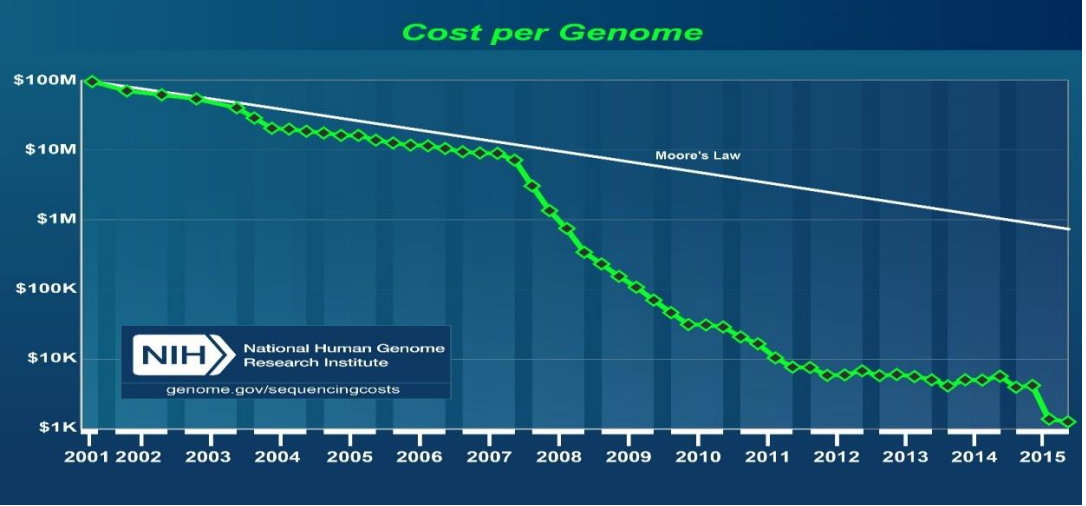
\includegraphics[width= 0.9 \columnwidth]{/Users/yu-pinglin/Desktop/Essay/6002.png}
    \centering
    \caption{Changes in the cost of sequencing over time}
\end{figure}
    
\section{PROBLEMS ASSOCIATED WITH BIG DATA IN BIOINFRMATICS}
\subsection{DATA STORAGE}
Since such amount of sequence data generated from hight throughout experimental technologies has introduced a new dimension and a blueprint for future biology and biomedical research, which provided an opportunity to discover a human mendelian disease is caused by which existence of a gene locus or mutations underlying a vast number of interesting mouse phenotype or perform gene-based pre-symptomatic prediction of illness in a shortest of processing time with access to a DNA sample and associated phenotypes in the public database. It is crucial to efficiently handle these data from a huge database. The storage and maintenance of Petabytes of data have strict requirements for storage and management. For some of the governmental organizations like NCBI or large private departments like yahoo, Facebook, etc, they might capable of storage such vast massive of data, on another side, this will pose a financial burden for some of the company to have such large scale storage and computational infrastructure, as the maintenance and implementing cost may be extremely high. During big data acquisition, heterogeneity issues may occur since the data are collected from multiple resources. To avoid redundancy and more effectively use the storage space, removing redundant or useless data are an indispensable process when researchers performed data analysis. Owing to the appearance of cloud computing, with the issue of data storage encountered in the personal storage system, Cloud computing has been widely utilized in the field of bioinformatics in response to the amount of data generation continues to expand at a tremendous rate, due to its superiority in elasticity, cost-effectively, smooth downgrading. 

\subsection{DATA TRANFER}
In most cases, the processing of a huge data, e,g 100 Gigabytes (GB) of haploid human genome transfer from one location to another is carried out primarily by the most convenient method to them: use of external hard disk or mail, physical drives, web-based service, FTP and so on, which is always very time consuming and hardware-demanding. With considerable effort and attention has been given to improving the long data transfer times, here come out several reliable resources with satisfying user experience, as they guarantee the data can be free from any loss and damage in the possible shortest of transfer time, for example, both of paralleling and grid computing are being the cost-effective and efficient of a method, as they can make use of computation resources by dividing large of tasks into the different processor. Each process will responsible for a small piece of work, giving back the integrated results generated from each process in the end.

\subsection{SECURITY}
With massive increase in data generation and comsumption then ever before, leading critical issues about retaining security of data ,as the big data mostly contains amount of personal information. Adoption of better security system, for example, Authenticated encryption wiht advcend encryption algorithms only allowing authorized user access to the data, to guard and monitor the processing of data flowing in and out is essentail to prevent them from attach , illegal theft or other spitful action that could pose great risk to the integraity and availability of data.Unfortunately, these are still insufficient protect our data apporiately.In ligth of this situation, there are great number of general security measurement that we can utilized by ourselves.
(i)Building up a strong firewell is the first line of defencse to keep your data protected. A firwall can be intergate into a physicall hardware device or software program.The benefit of the firewall is rountiely manage and monitor the network traffie, serving as an important barricade to stop and detect any hackers or virus which are inlcine to sneak into your system without permsssion.
(ii) Implement effective safeguard policy and safety measurement (developing a tiered access system) to ensure no sensitive data leakage and reduce the opportunity of any unauthorized users approch data from exterior or interior sources to steal wisdom.

 
\section{CONCLUSION}
Big data has affected all work of life, for bioinformatic filed which empower enormous of opportunity for us to look at the biological information underlying the diverse organisms including animals, plants, and microbes in a  more broad perspective(such as in the areas of drug development and personal medicines).On the other hand, the scientist has faced difficulty in dealing the increasing amounts of omics data, dut to the processing speed of the Internet and the accommodation of computers does not meet the need to analysis, transfer and integrity of biological data, besides, the problem of security, privacy and ethical issues also present challenge for biology community. To make the bioinformatics field more productive and flourishing, we certainly need the coordinated efforts from both experimental and computational biologists on the improvement of computational methods, infrastructure scalability, and efficient algorithms to keep up with the growth rate of big data.

\medskip


\emergencystretch=1em
\printbibliography[title=Reference]

\end{document}